\section{Use Case Diagrams}
A UML use case diagram is the principal form of system/software requirements for an underdeveloped software program\textsuperscript{[7]}.

\subsection{Global Use Case}
The global use case diagram offers a bird's-eye view of the UNInest platform, showing how each actor—Student, Owner, and Administrator—engages with core system functions.

\begin{figure}[H]
    \centering
    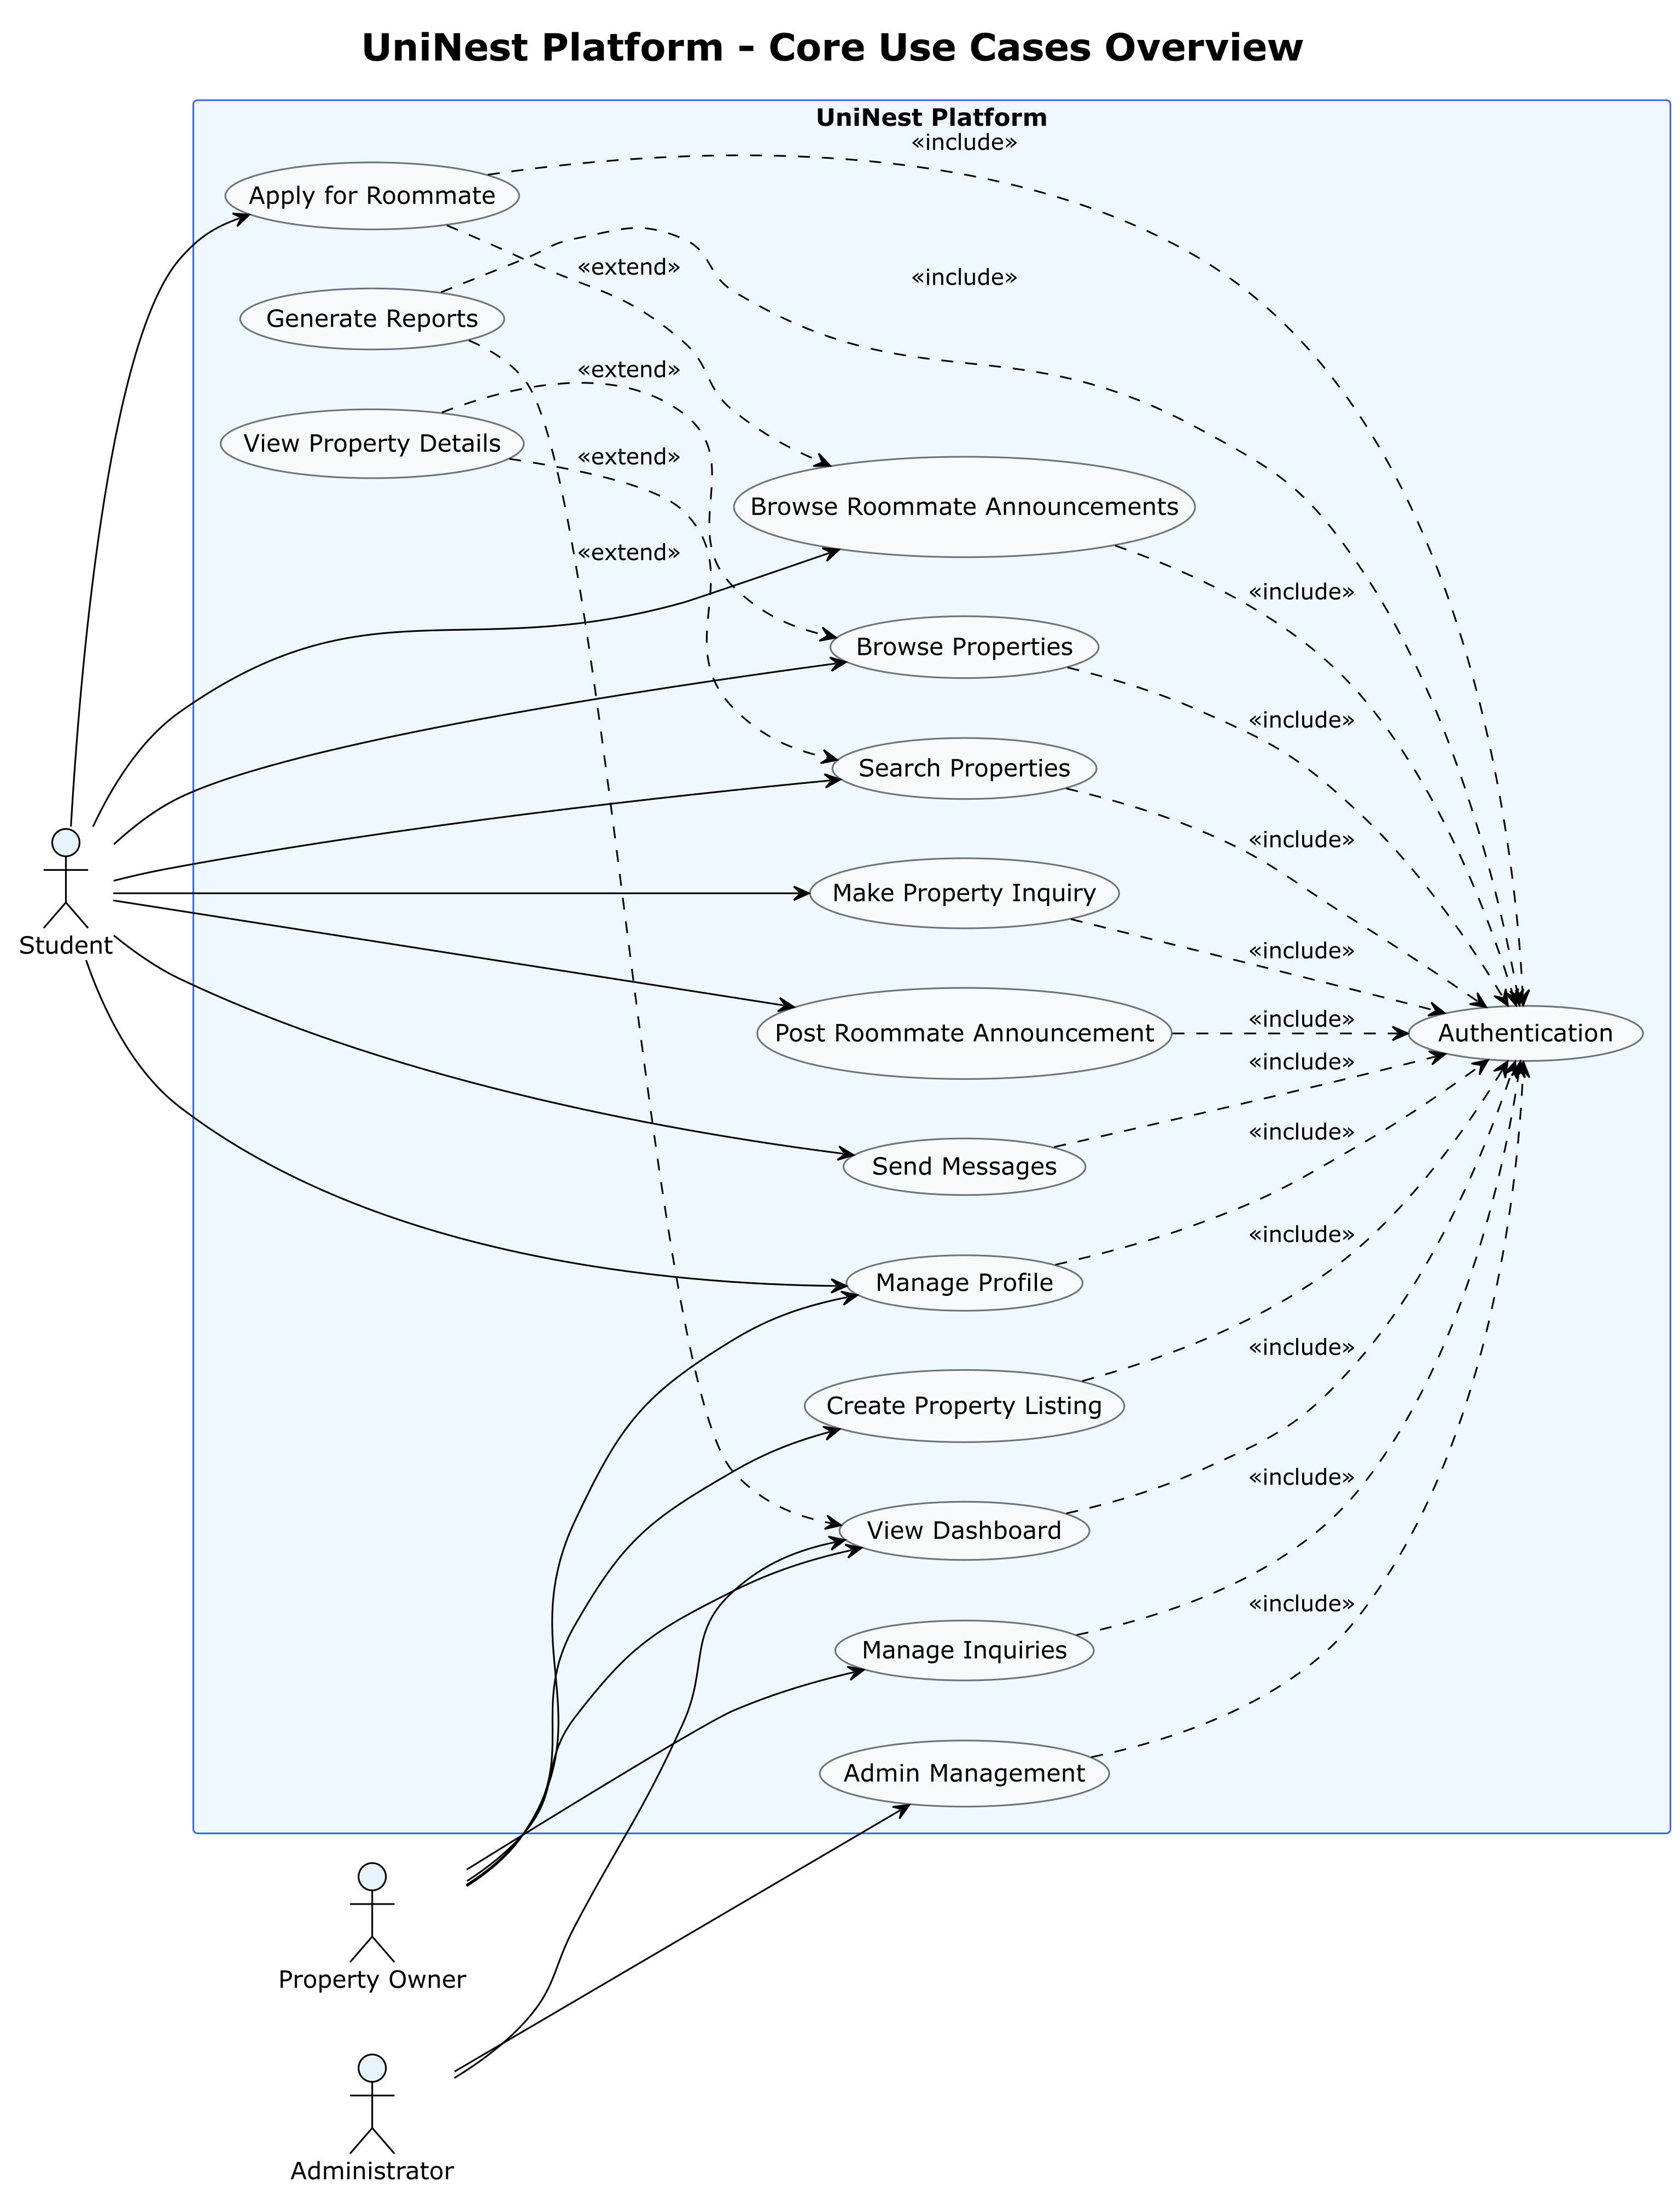
\includegraphics[width=0.85\textwidth]{global use case.jpg}
    \caption{Global Use Case Diagram}
    \label{fig:global_use_case}
\end{figure}

\subsection{Admin Use Case}
This diagram outlines all interactions available to the Admin, including full control over users, property listings, roommate announcements, and overall control.

\begin{figure}[H]
    \centering
    \includegraphics[width=0.8\textwidth]{adminusecase.jpg}
    \caption{Admin Use Case Diagram}
    \label{fig:admin_use_case}
\end{figure}

\subsection{Student Use Case}
This diagram outlines the interactions available to a Student user in the UNInest platform. Students can register, search for housing, filter listings, and contact property owners. They also have the ability to manage their profiles and benefit from the roommate recommendation portal.

\begin{figure}[H]
    \centering
    \includegraphics[width=0.9\textwidth]{student.jpg}
    \caption{Student Use Case Diagram}
    \label{fig:student_use_case}
\end{figure}

\subsection{Owner Use Case}
This use case diagram outlines the interactions available to the Owner on the UNInest platform. Owners can register and manage their listings, including adding new properties, updating existing details, viewing inquiries from students, and accessing their dashboards.

\begin{figure}[H]
    \centering
    \includegraphics[width=0.9\textwidth]{owner.jpg}
    \caption{Owner Use Case Diagram}
    \label{fig:owner_use_case}
\end{figure} 